\section{Auswertung}
\label{sec:Auswertung}
%Siehe \autoref{fig:plot}!

\subsection{Moden}
In diesem Teil werden die Moden mithilfe eine Oszilloskop untersucht.
Die aufgenommenen Werte zu zu den Moden sind in \autoref{tab:moden_messwerte} gelistet.
%tabelle messwerte
\begin{table}
    \centering
    \caption{Messwerte zu den drei Moden, wobei der erste Wert das Maximum beschreibt und die anderen beiden den Punkt links bzw. rechts vom Maximum bei dem die Spannung die hälfte des Maximums beträgt.}
    \begin{tabular}{c c c}
        \toprule
        Modennr. & $U \,/\, V$ & $A \,/\, V$ \\
        \midrule
        1 & $220$ & $31.25$ \\
        & $205$ & $15.625$ \\
        & $240$ & $15.625$ \\
        \hline
        2 & $140$ & $21.25$ \\
        & $120$ & $10.625$ \\
        & $150$ & $10.625$ \\
        \hline
        3 & $85$ & $17$ \\
        & $70$ & $8.5$ \\
        & $95$ & $8.5$ \\
        \bottomrule
    \end{tabular}
    \label{tab:moden_messwerte}
\end{table}
\FloatBarrier
Es liegt ein vollständig bestimmtes LGS vor mit drei Punkten je Mode vor.
Eine Moden wird durch eine Parabel
\begin{equation*}
    y_i = x \cdot U_i^2 + y \cdot U_i + z
\end{equation*}
beschrieben, wobei $x, y, z$ die zu bestimmenden Parameter und $y_i, U_i$ die gemessenen Datenpunkte sind.
Das LGS ist trivial zu lösen und wird hier nicht weiter ausgeführt.
Die Lösung kann in \autoref{fig:moden} graphisch und in \autoref{tab:moden_ergebnisse} quantitativ betrachtet werden.
\begin{figure}
    \centering
    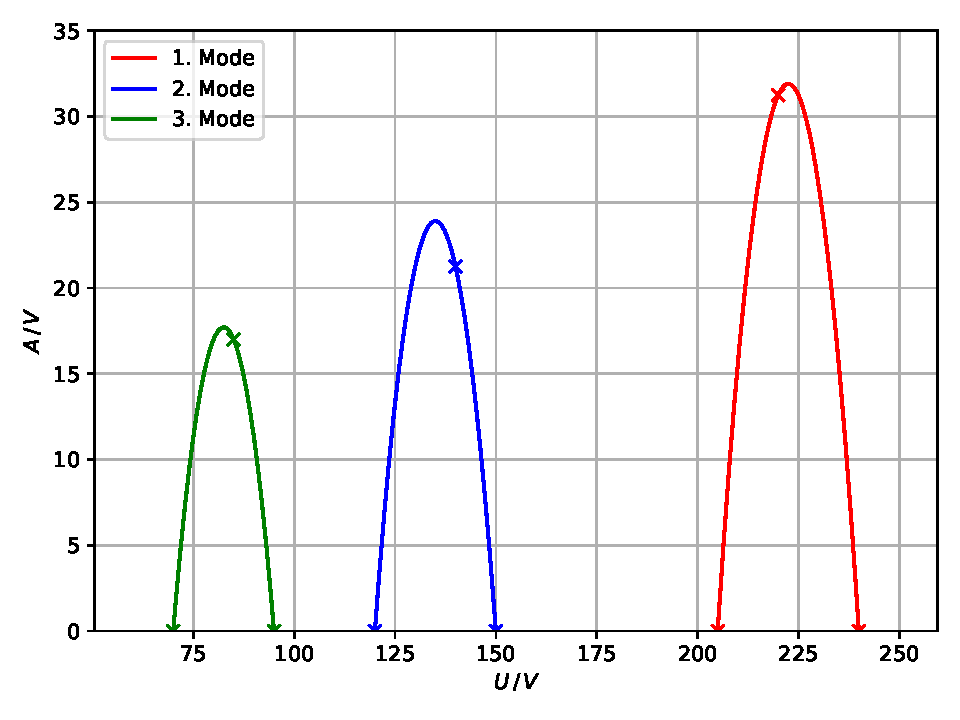
\includegraphics[width=0.8\textwidth]{content/data/moden.pdf}
    \caption{Die Messwerte $x$ mit zugehöriger Fit-Kurve (Ausgleichsparabel) für die drei Moden. \cite{matplotlib}\cite{numpy}}
    \label{fig:moden}
\end{figure}

%tabelle ergebnisse
\begin{table}
    \centering
    \caption{Die Parameter $x, y, z$, die die Ausgleichsparabel für eine Mode beschreiben.}
    \begin{tabular}{c c c c}
        \toprule
        Modennr. & $x$ & $y$ & $z$ \\
        \midrule
        1 & $-0.052$ & $23.177$ & $-2546.875$ \\
        2 & $-0.053$ & $14.344$ & $-945.625$ \\
        3 & $-0.057$ & $9.35$ & $-368.333$ \\
        \bottomrule
    \end{tabular}
    \label{tab:moden_ergebnisse}
\end{table}

\subsection{Bestimmung der Frequenz und Phasengeschwindigkeit im Hohlleiter}
